 %Diese Zeile bitte -nicht- aendern.
 \documentclass[course=erap] {aspdoc}

 %eigene Imports
 \usepackage{amsfonts}
 \usepackage{pgfplots}
 \usepackage{ulem}
 \usepackage{amssymb}
 \usepackage{mathtools}
 \usepackage{graphicx}
 \pgfplotsset{compat=1.16}
 
 
 %%%%%%%%%%%%%%%%%%%%%%%%%%%%%%%%%
 %% TODO: Ersetzen Sie in den folgenden Zeilen die entsprechenden -Texte-
 %% mit den richtigen Werten.
 \newcommand{\theGroup}{233} % Beispiel: 42
 \newcommand{\theNumber}{A316} % Beispiel: A123
 \author{Ludwig Gröber \and Julian Pins \and Daniel Safyan}
 \date{Sommersemester 2023} % Beispiel: Wintersemester 2019/20
 %%%%%%%%%%%%%%%%%%%%%%%%%%%%%%%%%
 
 % Diese Zeile bitte -nicht- aendern.
 \title{Gruppe \theGroup{} -- Abgabe zu Aufgabe \theNumber}
 
 \begin{document}
     \maketitle
 
 
     \section{Einleitung}
     In den Bereichen der Control-Theory und Datenverarbeitung gibt es zahlreiche Anwendungen, in denen die Berechnung bestimmter mathematischer Funktionen von großer Bedeutung ist. Eine dieser Funktionen ist der \textit{Areasinus Hyperbolicus} ($arsinh(x)$), der unter anderem die Beschreibung nichtlinearer Beziehungen und Modellierung von Sättigungsprozessen ermöglicht. Um die Genauigkeit und Effizienz solcher Berechnungen zu garantieren, ist es von entscheidender Bedeutung, die Berechnung des $arsinh(x)$ effizient umzusetzen.  
          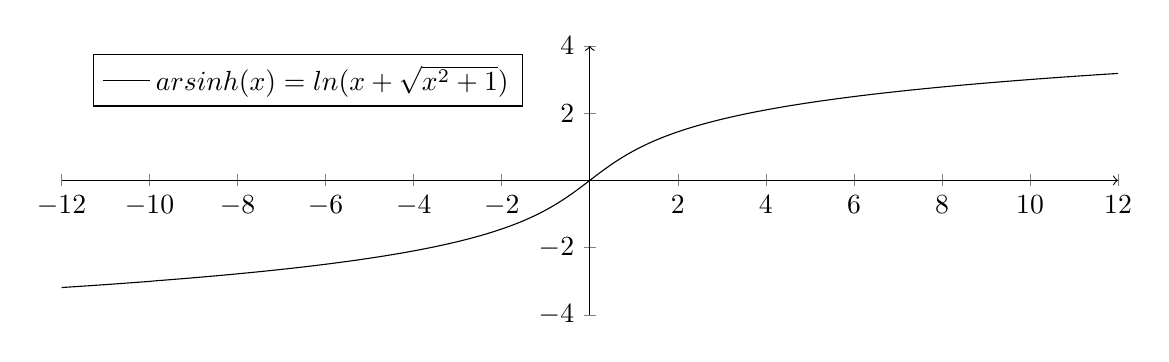
\begin{tikzpicture}
         \begin{axis}[
             legend pos = north west,
             width = 15 cm,
             height = 5 cm,
             xmin = -12, xmax = 12,
             ymin = -4, ymax = 4,
             axis lines=middle, 
             axis line style={->},
             domain= -20: 20,
             samples = 500
             ]
             \addplot[] {ln(x + sqrt(x*x+1))};
             \legend{$arsinh(x) = ln(x + \sqrt{x^2 + 1})$}
             
         \end{axis}
     \end{tikzpicture}
     
 
 
 
     \subsection{Analyse und Spezifikation der Aufgabenstellung}
     Unsere Aufgabe ist eben diesen $arsinh(x)$ zu approximieren.
     Genauergesagt verlangt die Aufgabenstellung explizit zwei Implementierungen, die nur auf einfachen arithmetischen Ausdrücken basiert sowie eine Vergleichsimplementierung, die komplexe Instruktionen benutzen darf. Eine dieser Implementierungen muss soll dabei eine reine Reihe sein, während die andere einen Tabellen-Lookup benutzen soll.
    
     Für unsere Implementierung haben wir folgende Annahmen getroffen.
     Mit der \textbf{"reinen"  Reihenentwicklung} bezeichnen wir eine Implementierung, welche mit exakt einer Reihendarstellung die Funktionswerte berechnet. Fallunterscheidungen nach Intervallen von x dürfen in dieser Implementierung also grundsätzlich nicht gemacht werden. Hierbei sollte also eine Reihe gewählt werden, deren Konvergenzbereich am ehesten für ein mögliches Anwendungsgebiet geeignet ist.
    
     Da die reine Reihenentwicklung nicht für alle Eingabewerte konvergiert haben wir eine Implementierung, die \textbf{mehrere Reihenentwicklungen für verschiedene Intervalle} der Eingabe verwendet. Es soll dennoch die Anzahl der Fallunterscheidungen minimal gehalten werden, indem  möglichst wenige verschiedene Reihenentwicklungen und eine feste Anzahl an berechneten Reihengliedern verwendet werden.
 
     Für die Implementierung der \textbf{Lookuptabelle} haben wir versucht nicht zu viel Speicherplatz zu verwenden, da für die meisten Anwendungen Speichereffizienz wichtig ist. Eine Abwägung zwischen Speicherplatz und Genauigkeit findet sich in Kapitel 2.2. Wir haben uns zudem für eine Lookuptabelle mit linearer Interpolation entschieden.
 
     Als \textbf{Vergleichsimplementierung} verwenden wir die arsinh(x) Funktion der C math Bibiliothek. Diese wird in erster Linie für die Bewertung der Genauigkeit zu Rate gezogen. Es sei an dieser Stelle bereits erwähnt, dass Funktionen der C-Mathematikbibliothek auf Maschinenebene implementiert sind bestimmte Hardwarefunktionen nutzen können. Daher wird diese Implementierung an Performanz kaum zu übertreffen sein.
 
     Diese vier Implementierungen sollen in Kapitel 3 und 4 auf Performanz und Genauigkeit untersucht, verglichen und anhand der Ergebnisse bewertet werden.
     
 
 
     \section{Lösungsansatz}
 
     Sowohl für die Implementierung mit einer Reihendarstellung, als auch für die Lookuptabelle haben wir uns die Punktsymmetrie der $arsinh$-Funktion zunutze gemacht: $arsinh(-x) = -arsinh(x)$. Die Funktionswerte für negative Eingabewerte, werden mit $-arsinh(|x|)$ berechnet. In der Folge wird daher vor allem der Fall $0\leq x$ betrachtet.

     \subsection{Reine Reihendarstellung}
     \subsubsection{Problematik und Ansätze}

     Bei der Interpolation durch eine "reine" Reihe der Form $\sum_{k=0}^{\infty} a_k x^k$ bzw. $\sum_{k=0}^{\infty} a_k x^-k$ stößt man unvermeidbar auf das problem von Overflows.
     Unabhängig welche Reihe man benutzt, entweder für sehr große Werte oder sehr kleine Werte von $x$ können die Zwischenergebnisse $x^{\pm k}$ nicht als $double$ dargestellt werden, obwohl das für das Endergebnis nicht gelten muss.
     Dadurch kommen wir auf Reihendarstellungen mit begrenzten Gültigkeitsbereichen.
     Wir versuchen also eine Reihenentwicklung zu finden, die für einen sinnvollen Konvergenzbereich möglichst genaue Ergebnisse liefert. Hierzu haben wir unter anderem die Methode der kleinsten Quadrate verwendet, um geeignet Koeffizienten für Reihenglieder mit positiven oder negativen Potenzen zu finden. Die auf diese Weise hergeleitete Reihenentwicklung liefert allerdings für Werte zwischen den verwendeten Datenpunkten sehr ungenaue Ergebnisse, da es sich bei der arsinh-Funktion nicht um ein lineares Modell handelt. Wir haben daher stattdess eine Reihenentwicklung für das Intervall $$$$ hergeleitet, die im folgenden näher erläutert werden soll.
     \subsubsection{Umsetzung}
     
     \[ \operatorname{arsinh}(x) =
     \begin{cases}
        \textit{TaylorArsinh}     & \text{ falls } |x| < 1 \\
        ln(2x) + error(x)  & \text{ falls } |x| >1 \\
        x     & \text{ falls } x \in \{\pm\inf, \pm Nan\}\\
    \end{cases}\]
    Für eine bessere Verständlichkeit werden wir nach diesem Kapitel die drei Reihen mit \textit{TaylorArsinh}, \textit{TaylorLn} und \textit{Restreihe} bezeichnen.
    Die Berechnungen sollen im Folgenden näher erläutert werden:
    
    \subsection{Reihendarstellung für $|x|\leq 1$}
     Für $|x| \leq 1$ wird die Taylor-Reihe des $arsinh(x)$ um den Entwicklungspunkt 0 verwendet:
     \[
        \textit{\textbf{TaylorArsinh}}\coloneqq arsinh(x) = \sum_{k = 0}^{\infty} \frac{(2k-1)!!(-x^2)^k}{(2k)!!(2k + 1)}
         = \sum_{k = 0}^{\infty} \frac{(-1)^k(2k)!x^{2k + 1}}{(2k + 1)(2^k*k!)^2}
     \]
     Durch das Auflösen der Doppelfakultäten entsteht eine deutlich leichter implementierbare Formel.
     %Da diese Reihe nur gültig ist für $|x| < 1$, werden für Werte außerhalb dieses Wertebereichs die anderen Reihen herangezogen.
     %x>1
     \subsection{Reihendarstellung für $|x|\geq 1$}
     Die Berechnung für $|x| > 1$ folgt aus folgender Näherung:
     \[
         arsinh(x) = \ln(x + \sqrt{x^2 + 1}) = \ln(2x) + error(x)
     \]
     Der Fehler dieser Näherung kann durch eine dritte Reihe berechnet werden, die vor allem für den Funktionswert von Eingabewerten $|x| < 2^{8}$ essentiell ist:
     \[
         \textit{\textbf{Restreihe}}\coloneqq error(x) =  \sum_{k = 1}^{\infty} \frac{(-1)^{k - 1}(2k)!}{2k(2^k\cdot k!)^2} \cdot \frac{1}{x^{2k}}
     \]
     
     Für die Berechnung von $\ln(2x)$ verwenden wir die Taylorreihe des natürlichen Logarithmus um den Entwicklungspunkt 1. Es gilt zu beachten, dass diese Reihe nur im Wertebereich $[0, 2]$ konvergiert.
     \[
         \textbf{\textit{TaylorLn}}\coloneqq\ln(x) = \sum_{k = 1}^{\infty} \frac{(-1)^{k + 1}}{k}(x - 1)^k
     \]
     Aufgrund der begrenzten Gültigkeit der Reihe machen wir uns bei der gemischten Implementierung das $double$ Datenformat zunutze machen, um die Berechnung zu optimieren. Durch eine Bitmaske lassen sich effizient Exponent und Mantisse von $x$ ermitteln. Mit Exponent und Mantisse lässt sich nun folgende Umformung treffen:
     \begin{gather*}
         x = M\cdot2^E \,\,\, mit \,\,\, M = implizierte Mantisse \,\,\, E = implizierter Exponent\\
         arsinh(x) \approx \ln(2x) = \ln(2) + \ln(x) = \ln(2) + \ln(M\cdot2^E) = \ln(2) + E\cdot\ln(2) + \ln(M)\\
     \end{gather*}
     Da $M\in[1, 2[$ liegt, kann nun \textit{TaylorLn} für die Berechnung von $\ln(M)$ verwendet werden. Da die Reihe bereits für wenige Reihenglieder exaktere Ergebnisse liefert, je näher der zu berechnende Wert an Eins liegt, haben wir uns dafür entschieden, alle Werte der Mantisse, die über $1.\overline{3}$ liegen, nochmal zu halbieren und stattdessen den Exponenten um 1 zu erhöhen. Es gilt damit $M\in[0.\overline{6}, 1.\overline{3}]$. 

     Bei unserer Hauptimplementierung jedoch benutzen wir die Folgende Umformung:
     \[
            arsinh(x)\approx ln(2x) + error(x) = ln(2) - ln(\frac{1}{x}) + error(x)
     \]
     Dadurch bekommen wir im Argument des natürlichen Logarithmus wieder einen Wert für den die \textbf{TaylorLn} gilt. Um nun die reine Reihe zu erhalten, werden die beiden Reihen zu einer vereinigt. Es lassen sich nämlich durch Ausmultiplizieren der ersten n Reihenglieder die Koeffizienten bestimmen und eine herkömmliche Reihe der Form $\sum_{k=0}^{n} a_k x^{-k}$ erstellen.

     Die Koeffizienten der einzelnen Reihenglieder zu berechnen ist jedoch extrem Laufzeitaufwendig, da insbesondere die Berechnung der Fakultät viel Zeit kostet. Daher lässt sich die Berechnung optimieren, indem die Koeffizienten aller drei Reihen bereits vor Runtime berechnet werden. Durch das Horner-Schema lässt sich nun die Reihe besonders effizient berechnen. 
     
 
     \subsubsection{Abwägung Genauigkeit und Performanz}
     Die Anzahl an benutzten Reihenglieder, entsteht aus einer Abwägung zwischen Performanz und Genauigkeit.
     Wie viele Reihenglieder berechnet werden müssen, um ein möglichst genaues Ergebnis zu erhalten, hängt von den Eingabewerten ab. Da die Reihenglieder aller drei Reihen immer kleiner werden, gilt: Je kleiner das letzte berechnete Reihenglied, desto genauer ist auch das Ergebnis.
     
     
     Wir betrachten zunächst \textit{TaylorLn}:
     In unserer Implementierung liegt der Eingabewert für die Reihe im Intervall $[0.\overline{6}, 1.\overline{3}]$. Aus der Formel für das k-te Reihenglied 
     \[ \frac{(x - 1)^k}{k}
     \]
     lässt sich errechnen, dass spätestens das 28. Reihenglied dieser Reihe für alle Eingabewerte im gegebenen Intervall $[0.\overline{6}, 1.\overline{3}]$ kleiner als $2^{-50}$ ist. Somit würden alle weitere Reihenglieder bei der Addition mit dem Restterm (wegen der Limitierung durch die Mantisse auf 52 bit) nahezu vollständig ausgelöscht werden. Wir setzen daher die Anzahl der zu berechnenden Reihenglieder dieser Reihe auf 27.  
     
     Betrachten wir nun \textit{TaylorArsinh}. Das k-te Reihenglied hat den Betrag
     \[
     \frac{(2k)!}{(2k + 1)(2^k*k!)^2}\cdot x^{2k+1}
     \]
     Aus dieser Formel lässt sich bereits ablesen, dass ein Reihenglied kleiner ist, je kleiner x ist. Die Reihe liefert demnach bereits mit weniger Reihengliedern genauere Ergebnisse, je näher x an 0 liegt. Setzt man versuchsweise bestimmte Werte von x in die Formel ein, so lässt sich feststellen, dass für x = 0.25 alle Reihenglieder ab dem etwa 13. Glied keinen Einfluss mehr auf das Endergebnis haben. Für x = 0.5 müssen hingegen 26 Reihenglieder berechnet werden. Für x = 0.99 sind wir bereits bei etwa 1500 Reihengliedern. 
     
     Für die \textit{Restreihe}, kann eine äquivalente Überlegung getroffen werden, die ebenfalls belegt, dass exponentiell mehr Reihenglieder benötigt werden, je näher x an 1 liegt.
     
     Wie man sieht, benötigt man für Eingabewerte nahe an 1 eine unverhältnismäßig hohe Anzahl an Reihengliedern für ein exaktes Ergebnis. Aufgrund dieses exponentiellen Wachstums, haben wir uns also dafür entschieden, die Anzahl der zu berechnenden Reihenglieder für \textit{TaylorArsinh} und \textit{Restreihe} bei 13 zu belassen und damit einen geringen relativen Fehler in den Intervallen $0.25<|x|<4$ in Kauf zu nehmen. 
     Das Gegenspiel von relativen Fehler und Performanz werden in den folgenden Kapiteln noch näher untersucht und belegt.
     
     Es sei an dieser Stelle erwähnt, dass sich ausgehend von diesen Untersuchungen eine weitere Optimierung umsetzen lassen würde, die (beispielsweise mithilfe des Exponenten des Eingabewertes) jeweils die Anzahl der nötigen Reihenglieder bestimmt und dann eben diese (falls die Anzahl kleiner als 13 ist) berechnet. Durch diese Optimierung würde unnötiger Overhead durch die Berechnung von Reihenglieder, die nichts am Endergebnis ändern, vermieden. Da wir die Fallunterscheidungen ausschließen wollten, haben wir allerdings auf diese Optimierung verzichtet.
 
 
     
     %\subsubsection{Problematik der "reinen" Reihenentwicklung}
 
     
     \subsection{Tabellen-Lookup}
     Die Lookuptabelle speichert einige vorberechnete Werte der $arsinh$-Funktion und interpoliert für die verbleibenden Werte linear zwischen den beiden nächstgelegenen Tabellenwerten.
     Bei der Implementierung galt es zunächst zwischen Speicherplatz der Tabelle und Genauigkeit des Ergebnisses abzuwägen. Um in einem realistisch umsetzbaren Rahmen zu bleiben, haben wir uns für ein Limit von 1 MB für die Lookuptabelle entschieden. Diese Größe ermöglicht das Speichern von etwa 40000 Werten. Wir haben uns für eine logarithmische Verteilung der Werte entschieden, da auch die Verteilung aller möglichen Werte im Datentyp $double$ logarithmisch ist. Für alle positiven Eingabewerte wurde für jeden möglichen Exponenten $[-1023, +1023]$ eine feste Anzahl an Werten vorberechnet. Durch unser Speicherlimit wurden wir hierbei auf 16 Werte pro Exponent beschränkt, wodurch insgesamt 32753 Werte gespeichert werden müssen. Die Ergebnisse für diese Designentscheidung werden im Kapitel Genauigkeit noch näher analysiert.
     
     Diese Verteilung ermöglicht zudem ein besonders effizientes Mapping der Eingabewerte auf den zugehörigen Index in der Lookuptabelle durch eine Hashfunktion. Durch eine Bitmaske lassen sich Exponent und die ersten 4 Bits der Mantisse ermitteln. Diese 15 bits bilden den Index des nächstkleineren Wertes, der in der Lookuptabelle liegt. Mit diesem und dem nächsten Tabellenwert, kann das Ergebnis nun linear interpoliert werden.
     Nachdem nun die Hashfunktion einen Index $i=hash(x)$ liefert, gilt: $table[i] \leq arsinh(x) \leq table[i+1]$. 
     Nun interpolieren wir in diesem Abschnitt linear mit $y_j = table[j]$:
     \[
         arsinh(x) \approx \frac{y_{i+1}-y_i}{\Delta x_{table}}\cdot (x-y_i) + y_i
     \]
     Da $\Delta x_{table}$ jedoch von $i$ abhängt, muss dieses erst bestimmt werden mit:
     \[
            \Delta x_{table} = x - x_i
     \]
     Dies geschieht durch eine Bitmaske sehr effizient.
     
     
 
 
 
     
     % Theoretischer Teil
     %In diesem Absatz rechtfertigen wir die beiden Ansätze der Reihenentwicklung und des Tabellen-Lookups mathematisch.
     %Sowohl die Polynominterpolation als auch die intervallweise lineare Interpolation sind
     % >>Leiten Sie mathematisch zwei Möglichkeiten her, die Funktion zu berechnen.
     % Verwenden Sie dazu sowohl eine reine Reihendarstellung als auch eine Methodik, die einen Tabellen-Lookup benutzt.
     % Ideen: Reihenentwicklung nicht zur Runtime, sondern zur Compiletime berechnen.
     % Runge Effekt: zwischen Integralgrenzen gut angenähert, wenn mit Polynom genähert wird. -> Deshalb funktioniert die Reihenentwicklung nicht.
     % Lösung: Splines über großen Bereich mit x^3 Polynom annähern. Intervall gleich verteilt. alpha x^3 + beta x^2 + gamma x + delta
     % Annäherung für große Werte: x^2 + 1 = x^2
     % Ableitung per Tailor-Reihe
     % Idee: 1. Chilliger Lookup Table mit Interpolation 2. Splines Lookup Table
     % Entwicklung als echte Reihendarstellung muss begrenzt werden im Wertebereich.
     % Grunstätzlich möglichst wenig zur Runtime berechnen.
     % Reihe: Basisfunktionen + Lineares Gleichungssystem
     % Lagrange Polynome
     % Tailor-Reihe / Tailor Entweicklung<<
 
     %\subsection{Implementierung mit komplexen Instruktionen}
 
     %Als Vergleichsimplementierung wurde eine weiter Funktion zu Rate gezogen, die komplexe Instruktionen der C-Math Bibiliothek verwendet. Die Verwendung solcher Instruktionen hat den Vorteil, dass dass die C-Math Bibiliothek hoch optimiert ist und somit sehr schnell ein exaktes Ergebnis liefern kann. Prinzipiell kann für die Berechnung die allgemeine Formel $ arsinh(x) = ln \left(x + \sqrt{x^2 + 1} \right)$ verwendet werden. Es kann allerdings bei der Berechnung von $x^2$ zu einem double Overflow kommen, falls x zu groß ist. Das ist genau dann der Fall, wenn $|x| > 2^{512}$, da dann $x^2 > 2^{1024}$ und damit außerhalb des durch double dargestellten Wertebereichs liegt. Damit für solche Werte nicht $+\inf$ zurückgegeben wird, verwenden wir für große x wie auch in der Reihenentwicklung die Näherung $arsinh(x)\approx ln(2x)$. Im Allgemeinen liefert diese Implementierung sehr exakte Werte. Eine Ausnahme stellen sehr kleine Werte dar, was im folgenden Abschnitt Genauigkeit noch näher erläutert werden soll.
 
     \section{Genauigkeit}
     Als Maßstab für die Genauigkeit unserer Ergebnisse wird im Folgenden der relative Fehler der Implementierung bezüglich des tatsächlichen mathematischen Funktionswert verwendet. Die folgenden Diagramme wurden erstellt, indem mithilfe einer C-Hilfsmethode für eine große Anzahl an Eingabewerten jeweils die Funktionswerte für alle drei Implementierungen brechnet und in Arrays gespeichert wurden. Anschließend wurden diese Funktionswerte in einem Python-Programm zu den jeweilgen relativen Fehlern ausgewertet und mithilfe der Bibiliothek matplotlib als Graph dargestellt.
 
     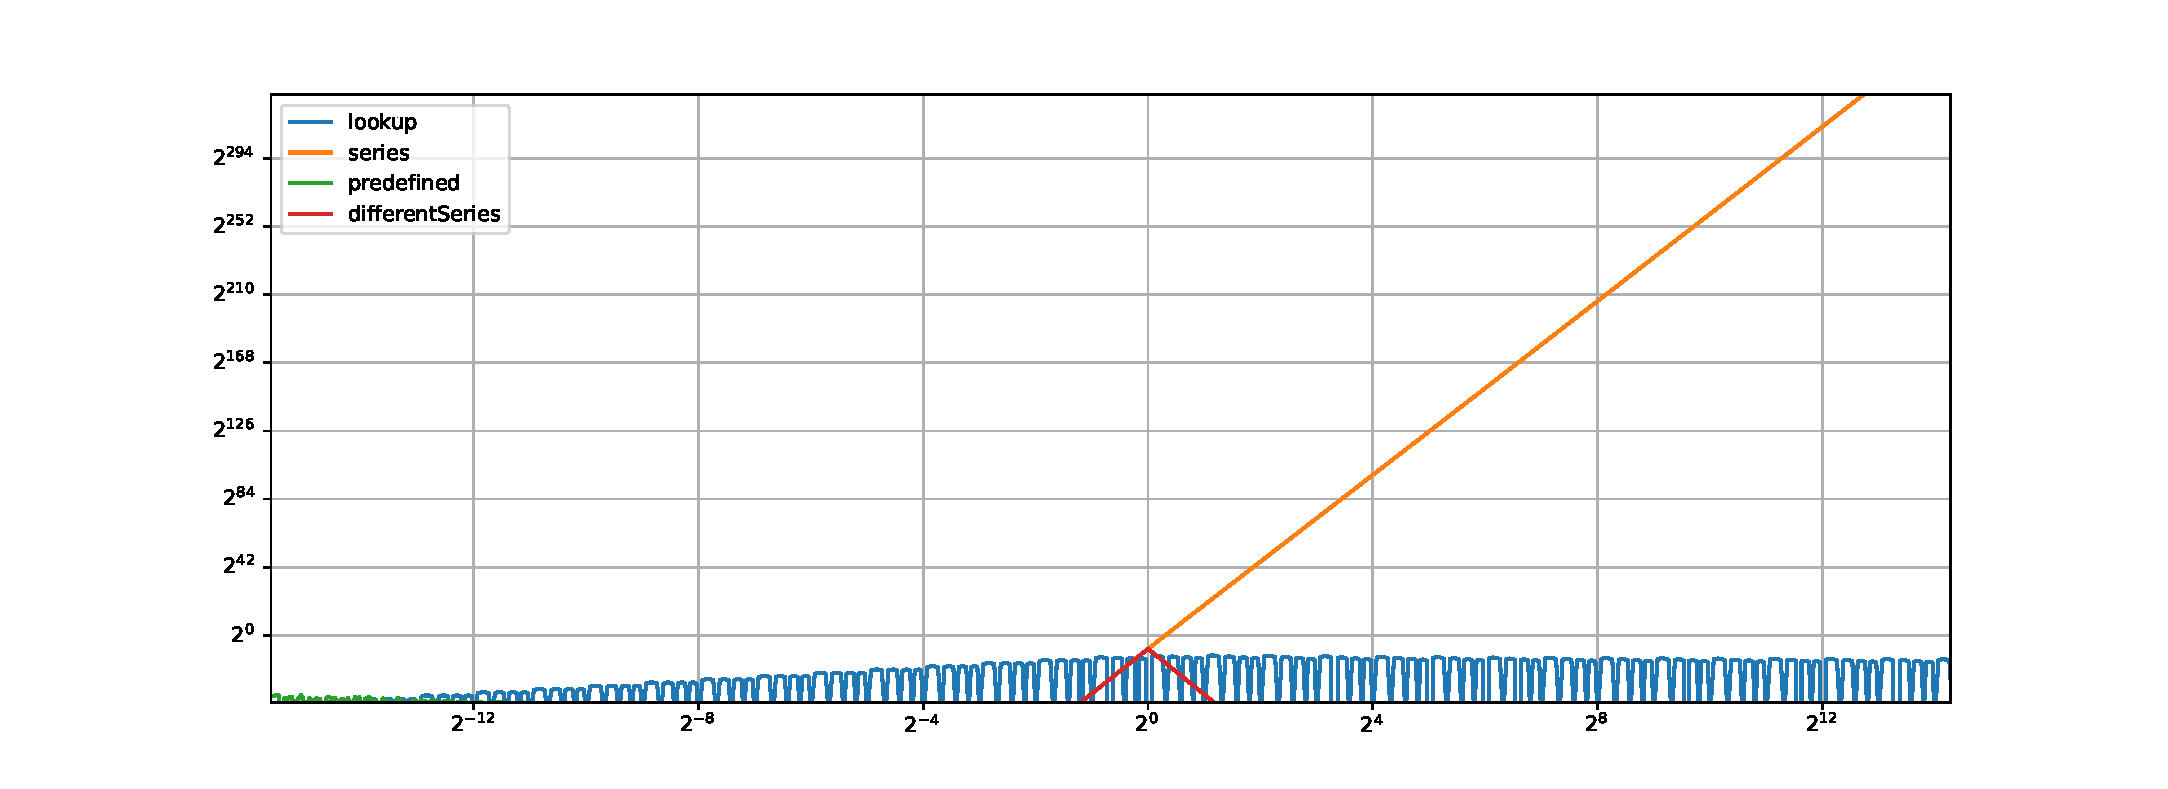
\includegraphics[scale = 0.17,]{Figure_1.png}
     \includegraphics[scale = 0.33,]{Figure_2.png}
     
     \subsection{Reine Reihenentwicklung}
     
 
 
     
     \subsection{Reihenentwicklung mit mehreren Reihen}
     Wie deutlich im ersten Diagramm erkennbar, liefert die Reihenentwicklung außerhalb der Intervalle $0.25<x<4$ nahezu immer den exakten Funktionswert. Es gibt einige Ausnahmen mit einem verschwindend geringen relativen Fehler $\leq2^{-50}$ , welche sich durch floating-point-Rundungsfehler bei der Umrechnung der Polynomkoeffizienten erklären lassen.
     Für einen Großteil der Eingabewerte liefert diese Funktion also tasächlich den genauest möglichen Funktionswert für den Datentyp double. Eine Ausnahme bildet jedoch das Intervall $0.25<|x|<4$. 
     
     Wie im zweiten (logarithmisch skalierten) Diagramm deutlich erkennbar, steigt der relative Fehler exponentiell an, je näher der Eingabewert an 1 liegt. Dies lässt sich  anhand der Konvergenz der Reihenglieder für verschiedene Eingabewerte erklären. Wie in Kapitel 2.1.1 erläutert, ist das Ergebnis genauer, je kleiner das letzte berechnete Reihenglied ist. Da wir für \textit{TaylorLn} die maximal nötigen Reihenglieder für double-Genauigkeit berechnen, hängen die Ungenauigkeiten mit \textit{Restreihe} und \textit{TaylorArsinh} zusammen. 
     Wir belegen zunächst, dass bei 13 Reihengliedern die Grenze für die Entstehung von Ungenauigkeiten in etwa bei 0.25 und 4 liegt. Hierzu berechnen wir jeweils das letzte Reihenglied für beide Werte 
     \[
     \textit{TaylorArsinh}: \frac{(2\cdot13)!0.25^{2\cdot13 + 1}}{(2\cdot13 + 1)(2^13\cdot13!)^2} \approx 2^{-59}
     \]
     \[
     \textit{Restreihe}: \frac{(2\cdot13)!}{2\cdot13(2^{13}\cdot 13!)^2} \cdot \frac{1}{4^{2\cdot13}} \approx 2^{-59}
     \]
     Da des letzte Reihenglied für beide Werte noch unter $2^{-52}$ liegt, hat das Ergebnis noch maximale double Genauigkeit. Für x-Werte näher an 1, wird jedoch das letzte Reihenglied immer größer, wodurch der relative Fehler exponentiell ansteigt. Wie im Graph zu sehen ist, hat die Reihenentwicklung ihren maximalen relativen fehler von circa $2^{-8} \approx 0.39\%$ am Eingabewert 1
     Berechnen wir jeweils das letzte (13.) berechnete Reihenglied für den Eingabewert 1 in den beiden Reihen so erhalten wir:
     \[
     \textit{TaylorArsinh}: \frac{(2\cdot13)!1^{2\cdot13 + 1}}{(2\cdot13 + 1)(2^13\cdot13!)^2} \approx 0.00574 \approx 2^{-8}
     \]
     \[
     \textit{Restreihe}: \frac{(2\cdot13)!}{2\cdot13(2^{13}\cdot 13!)^2} \cdot \frac{1}{1^{2\cdot13}} \approx 0.00596 \approx 2^{-8}
     \]
     Da das letzte Reihenglied die Größenordnung $2^{-8}$ hat, liegt auch der relative Fehler etwa in dieser Größenordnung. Der Graph bestätigt somit unsere Überlegungen zur Genauigkeit der Reihenentwicklungen. 
     
     
     \subsection{Lookuptabelle}
     Die Genauigkeit des Ergebnisses bei der Verwendung der Lookuptabelle hängt stark von den Eingabewerten ab. Ist der Eingabewert exakt einer der vorgespeicherten Werte in der Tabelle, so liefert die Funktion logischerweise das exakte Ergebnis. Am ungenauesten ist die Funktion für Eingabewerte, die genau zwischen zwei gespeicherten Tabellenwerten liegen. Das lässt sich deutlich an der großen vertikalen Streuung der Fehlerwerte erkennen.
     
     Im ersten Diagramm ist zudem deutlich erkennbar, dass die Funktion wie auch die Reihenentwicklung deutlich ungenauere Ergebnisse für Eingabewerte nahe an 1 liefert. Dies lässt sich mithilfe des Krümmungsverhaltens der Funktion begründen. Der folgende Graph zeigt die zweite Ableitung des $arsinh''(x) = \frac{-x}{x^2\cdot \sqrt{x^2+1}+\sqrt{x^2+1}}$
 
     
     \begin{tikzpicture}
         \begin{axis}[
             width = 15 cm,
             height = 5 cm,
             xmin = -10, xmax = 10,
             ymin = -0.5, ymax = 0.5,
             axis lines=middle, 
             axis line style={->},
             domain= -20: 20,
             samples = 500,
             ]
             \addplot[] {-x/((x*x)* sqrt((x*x)+1) + sqrt((x*x)+1))};
             \addplot [color=blue, mark = *] coordinates {
                 (-0.707106781093, 0.3849001794598)
             };
             \addplot [color=blue, mark = *] coordinates {
                 (0.707106781093, -0.3849001794598)
             };
         \end{axis}
     \end{tikzpicture}
 
     Wie man sieht, hat der $arsinh(x)$ eine maximale Krümmung bei circa $\pm 0.707$. Dementsprechend wird auch eine lineare Interpolation im Bereich dieser Stellen eine maximale Ungenauigkeit aufweisen.
     
     \subsection{Implementierung mit komplexen Instruktionen}
     Wie im ersten Diagramm zu sehen liefert die Implementierung mit komplexen mathematischen Instruktionen der C-Math Bibliothek für den Großteil des Wertebereichs den genauest möglichen Funktionswert für den Datentyp double. Eine Ausnahme bilden sehr kleine x-Werte. Dies lässt sich mit der Absorption beziehungsweise Auslöschung von bits begründen, welche bei der Addition von doubles unterschiedlicher Größenordnung unvermeidbar auftritt. Betrachten wir nun zunächst den Term $\sqrt{x^2 + 1}$ der allgemeinen Gleichung für den $arsinh(x)$. Ab $|x|<2^{-26}$ gilt stets $x^2<2^{-52}$. $x^2$ wird damit bei der Addition mit 1 vollständig absorbiert und $\sqrt{x^2 + 1}$ evaluiert zu 1. Hierdurch entsteht ein für kleinere $x$ immer größerer relativer Fehler. Ab $|x|<2^{-52}$ wird zudem x bei Addition auf 1 immer absorbiert, wodurch $\ln{(x+\sqrt{x^2 + 1})}$ automatisch zu 0 evaluiert. Für $|x|<2^{-52}$ ist die Implementierung mit komplexen mathematischen Instruktionen demnach kaum noch anwendbar, da das Ergebnis (mit Ausnahme von 0) immer einen relativen Fehler von $100\%$ haben wird.
     
     \section{Performanzanalyse}
     Die Performanz der Implementierungen wird anhand der Laufzeit gemessen.
     Diese wird im Folgenden mit der Libaray $time.h$ gemessen.
 
     \subsection{Methodik und Annahmen 0,5Seite}
 
     %Voraussetzungen
     Gemessen wurde auf einem System mit Intel i5-10210U Prozessor, 1.60 GHz, 8 GiB Arbeitsspeicher, Ubuntu 22.04.2 LTS, 64 Bit, 5.19.0-46-generic Linux-Kernel.
     Kompiliert wurde mit GCC 11.3.0 mit der Option -O3. Um eine optimale Vergleichbarkeit der Ergebnisse zu garantieren, wurden alle nicht für das Betriebssystem nötigen Prozesse beendet. 
 
     Da die Reihenentwicklung zwei sehr verschiedene Berechnungen für $|x|>1$ und $|x|\geq 1$ durchführt, wurden bei der Laufzeitmessung diese beiden Fälle unterschieden.
     Ansonsten hängt die Laufzeit aller drei Implementierungen nur bedingt von der Größenordnung der Eingabewerte ab, daher wurde die Laufzeitmessung für die beiden Intervalle jeweils mit repräsentativen Werten verschiedener Größenordnungen durchgeführt.
     Die Methoden wurden mit 10 verschiedenen Werten jeweils 100.000.000 mal aufgerufen, um dann das arithmetische Mittel der Zeit für einen Funktionsaufruf zu ermitteln.
 
     \subsubsection{Zeitmessung der Implementierungen}
 
     Der folgende Graph zeigt die durchschnittliche Laufzeit eines Funktionsaufrufes der drei Implementierungen mit Reihenentwicklung, Tabellen-Lookup und der Implementierung mithilfe komplexer Instruktionen der C-math-library in Nanosekunden:
 
     %Tabelle
     \begin{tikzpicture}
         \begin{axis}
             [
             ybar,
             width = 10 cm,
             height= \axisdefaultheight,
             bar width = 0.3 cm,
             enlarge x limits = {abs = 1.5 cm},
             symbolic x coords = {Reihe, Lookup,  predefined},
             xtick={Reihe, Lookup, predefined},
             ylabel={Zeit in ns},
             xlabel={Implementierung},
             legend style={at={(0.6, 0.9)},
               anchor=north,legend columns=-1},
             xtick=data,
             nodes near coords,
             nodes near coords align={vertical},
             bar width = 0.9cm,
             ]
             \addplot coordinates {(gemischte Reihe, 6.369) (reine Reihe,6.369) (Lookup, 2.613) (predefined, 0.0)};
             \addplot coordinates {(gemischte Reihe, 29.212) (reine Reihe, 6.369) (Lookup, 2.613) (predefined, 1.648)};
             \legend{$|x|<1$  ., $|x|\geq 1$}
         \end{axis}
     \end{tikzpicture}
 
     \subsection{Bewertung, Einordnung und Erklärung der Ergebnisse}
     %Folgerungen
     Wie in der Abbildung zu sehen ist, ist die reine Reihen-Implementierung um ein Vielfaches (bis zu 12x) langsamer als die anderen
     beiden Vergleichsimplementierungen.
     Hier liegt die Stärke einer Implementierung durch Lookup-Tabelle, da wir hier für jeden
     Input nur sehr billige arithmetische Ausdrücke zum linearen Interpolieren verwenden.
     Die Reihenentwicklung andererseits verwendet viel mehr Multiplikationen und Summen über mehrere Iterationen, was jedoch als Reihendarstellung mit Polynomen nicht zu vermeiden ist.
     
 
     \section{Zusammenfassung und Ausblick}
     \subsection{Zusammenfassung}
     Zusammenfassend lässt sich feststellen, dass der Trade-off zwischen Performance, Genauigkeit und Speicherverbrauch für die beiden Implementierungen mit einem Tabellenlookup beziehungsweise einer Reihenentwicklung sehr unterschiedlich ist.
     Der Tabellenlookup ist zwar sehr schnell, benötigt allerdings auch immer mehr Speicherplatz, je genauere Werte man erhalten möchte.
     In unserer Implementierung, die insgesamt ca. 30000 Werte in einer Lookuptabelle speichert, hat die Berechnung einen maximalen relativen Fehler von bis zu etwa 0.01 Prozent.
 
     Die Reihenentwicklung auf der anderen Seite liefert für etwa 49.4\% aller doubles den exakten Funktionswert, wird allerdings für Eingabewerte nahe an Eins ungenau - um das exakte Ergebnis für Eins zu erhalten wäre eine unvertretbar hohe Anzahl an Reihengliedern erforderlich, die zu extremen Performanzeinbußen führen würden. Da jedoch der interessanteste Bereich über 1 hinausgeht, lässt sich schließen, dass die Nutzung einer reinen Reihe, egal ob man die für $|x|\geq1$ oder $|x|\leq1$ verwendet, für diese Aufgabe nicht geeignet ist.
     Die gemischte Reihe liefert für 99,8\% aller doubles den exakten Funktionswert.
     Auch für die 27 reihenglieder der ln-Taylorreihe und die 13 Reihenglieder der beiden anderen Reihen, für die wir uns entschieden haben, benötigt die Reihenentwicklung für $|x|>1$ bis zu 11 mal so lange für die Berechnung, benötigt dafür aber auch über 600-mal weniger Speicherplatz für eine genaue Berechnung.
 
 
     
     \subsection{Anwendung}
     Welches Programm verwendet werden sollte, hängt von den Rahmenbedingungen ab.
     Der Areasinus Hyperbolicus findet in erster Linie Anwendung in verschiedensten Bereichen der Physik und Ingenierswissenschaften.
     Für die Auswertung großer Messreihen eignet sich die Lookuptabelle deutlich besser, da Messungen in der Regel sowieso einen kleinen Fehler aufweisen und die Lookuptabelle für viele Werte aufgrund der besseren Performanz schneller Ergebnisse liefert.
     Hat jedoch die exakte Genauigkeit der Ergebnisse ein höhere Priorität, so eignet sich die Reihenentwicklung mit einer geeigneten Menge an Reihengliedern deutlich besser.
 
     \subsection{Ausblick}
 
     In unserer Implementierung des $arsinh(x)$ haben wir uns auf eine reine Reihenentwicklung und eine einfache Lookup-Tabelle mit linearer Näherung beschränkt.
     Unter weniger strengen Rahmenbedingungen ließe sich die Implementierung allerdings sowohl in Bezug auf Laufzeit, als auch Genauigkeit noch signifikant optimieren. 
     
     Ein möglicher Ansatz ist die Verwendung von Splines in der Lookup-Tabelle: Statt der bisher linearen Näherung zwischen zwei Messpunkten in der Lookup-Tabelle, könnte man den $arsinh(x)$ in diesem Intervall durch eine Kurve annähern.
     Hierzu werden in der Regel Polynome vom Grad drei verwendet.
     Dadurch verbessert sich die Genauigkeit, insbesondere für x-Werte die genau zwischen zwei Werten in der Lookup-Tabelle liegen deutlich, während sich die Laufzeit nur minimal erhöht.
     Dafür steigt allerdings der benötigte Speicherplatz, da nun für jedes Intervall ein Polynom gespeichert werden muss.
     
     Eine mögliche weitere Verbesserung des Lookup-Tables ist eine effizientere Verteilung der Tabellenwerte. Dadurch dass wir nämlich linear zwischen den 
     werten interepolieren entsteht umso mehr Ungenauigkeit umso stärker sich die Steigung der Funktion ändert. Diese Steigungsänderung lässt sich mit der Krümmung messen.
     Diese ist für kleine x besonders hoch und sinkt immer weiter für betragsmäßig große Inputs. Deswegen würde man an Genauigkeit gewinnen können, ohne mehr 
     Speicher aufzuwenden, wenn man eine Mappingfunktion finden würde, die jedem x effizient den richtigen Tabelleneintrag zuorden kann.
      Ein weiterer Ansatz wäre, eine Kombination aus Reihenentwicklung und Lookuptabelle zu verwenden: 
     Wie zuvor beobachtet liefert die Berechnung mit einer Reihenentwicklung für x-Werte, die nicht nahe an Eins liegen, besonders genaue Ergebnisse. Für |x|<0.125 brauchen wir beispielsweise nur 13 Reihenglieder, für |x|>8 brauchen wir 13 Reihenglieder der Restreihe, sowie bis zu 33 Reihenglieder der Taylorreihe für ein exaktes Ergebnis. In diesen Intervallen bietet es sich also durchaus an eine reine Reihenentwicklung zu verwenden. In dem Intervall 0.125<=|x|<=8 braucht man allerdings mehr Reihenglieder, wodurch es zu Performanzeinbußen kommt. Es wäre demnach sinnvoll in diesem Intervall eine Lookuptabelle zu verwenden. Da der Wertebereich nun deutlich kleiner ist, lassen sich bereits in kleinen Lookuptabellen, deutlich exaktere Werte speichern, wodurch der maximale relative Fehler minimal gehalten wird. Dieser Ansatz zielt besonders auf die Genauigkeit des Ergebnisses ab. Durch die Verwendung einer Lookuptabelle erhöht sich zudem die Performanz, da für die verbleibenden x-Werte weniger Reihenglieder berechnet werden müssen, um ein exaktes Ergebnis zu erhalten. 
 
     Anzumerken ist zudem, dass sich insbesondere die Reihenentwicklung durch die Verwendung von Assemblerinstruktionen noch signifikant auf Laufzeit optimieren lässt. 
 
 % TODO: Fuegen Sie Ihre Quellen der Datei Ausarbeitung.bib hinzu
 % Referenzieren Sie diese dann mit \cite{}.
 % Beispiel: CR2 ist ein Register der x86-Architektur~\cite{intel2017man}.
     \bibliographystyle{plain}
     \bibliography{Ausarbeitung}
 % Sämtliche in der Ausarbeitung verwendeten Quellen sind hier aufzuführen.
 % Es sollen nur zitierfähige Quellen verwendet werden. Wir empfehlen die Verwendung von BibTEX.
 
 \end{document}